\section{Architettura}

\subsection{Introduzione}
\par Il prodotto ChatSQL è basato su un'architettura client-server. Il client è l'interfaccia attraverso la quale gli utenti interagiscono con il sistema, come ad esempio un browser web. In altre parole, il client è il componente che richiede risorse o servizi. Il server è l'applicazione che riceve ed elabora le richieste provenienti da uno o più client, fornendo risposte appropriate.

\begin{figure}[H]
  \centering
  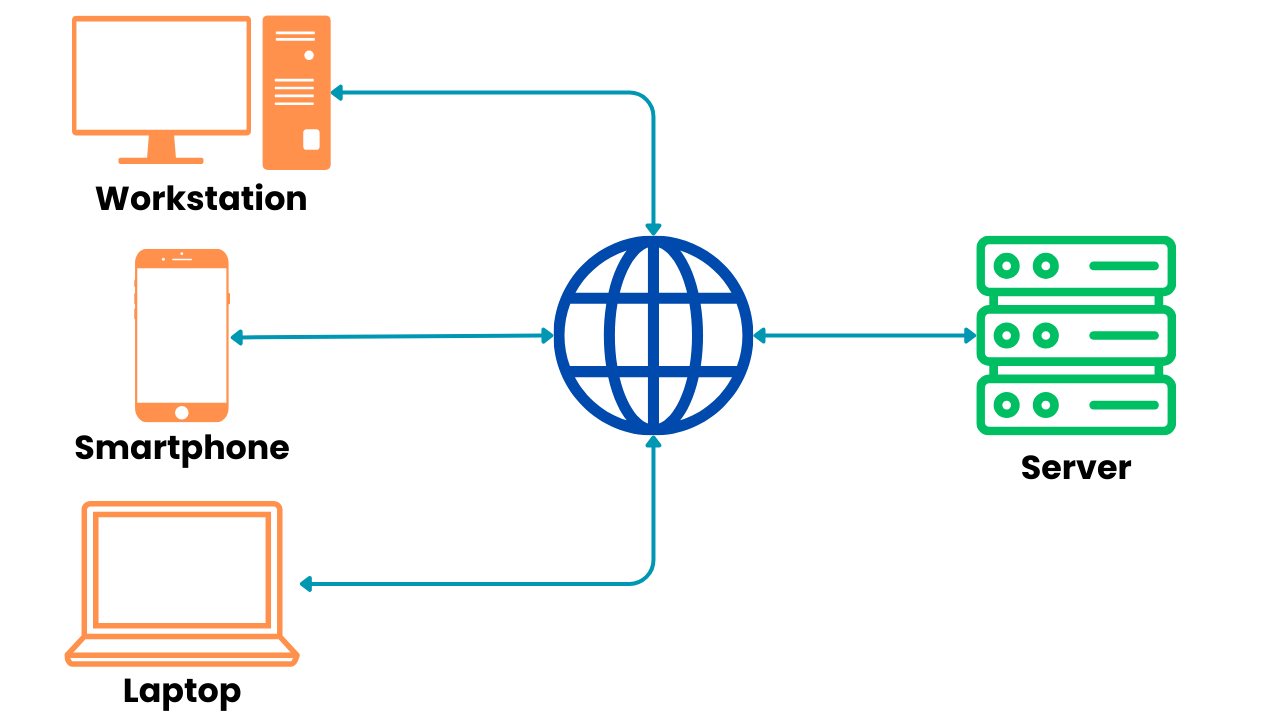
\includegraphics[width=0.95\textwidth]{assets/client_server.png}
  \caption{Architettura client-server}
\end{figure}

\par Per migliorare lo sviluppo collaborativo, la modularità e la manutenibilità, il sistema è stato suddiviso in due componenti principali:
\begin{itemize}
  \item \textbf{Front-end}: è la porzione di un sistema che l'utente visualizza e con cui può interagire. Il front-end è sviluppato utilizzando il framework \glossario{Vue.js} ed è responsabile dell'interfaccia grafica, che deve essere intuitiva, funzionale e accattivante. Trasmette le richieste dell'utente al back-end e visualizza i risultati ottenuti;
  \item \textbf{Back-end}: è il segmento che gestisce la logica di business, l'elaborazione dei dati e la comunicazione con i database e altri servizi. Il back-end è sviluppato utilizzando il framework \glossario{FastAPI}.
\end{itemize}

\vspace{0.5\baselineskip}
\par La comunicazione tra il front-end e il back-end avviene tramite chiamate \glossario{API}. Il team segue le linee guida e i principi definiti da REST (representational state transfer), uno stile architetturale che impone condizioni sul funzionamento di un'API. Le REST API (o RESTful API) sono stateless, il che significa che ogni richiesta HTTP deve includere tutte le informazioni necessarie per elaborarla. Questo riduce il carico sul server e migliora la scalabilità. Inoltre, l’approccio stateless agevola l'implementazione di sistemi di caching, migliorando le prestazioni complessive. Una REST API è simile a un sito web in esecuzione in un browser con funzionalità HTTP integrata. Le operazioni sono basate su metodi HTTP standard come GET, POST, PUT e DELETE.

\vspace{0.5\baselineskip}
\par La persistenza delle informazioni dei dizionari (nome, descrizione, ecc.) è garantita dalla presenza di un database, che memorizza anche gli operatori registrati nel sistema. Il database è implementato utilizzando SQLite. Di seguito è riportata l'architettura ad alto livello della web app.

\begin{figure}[H]
  \centering
  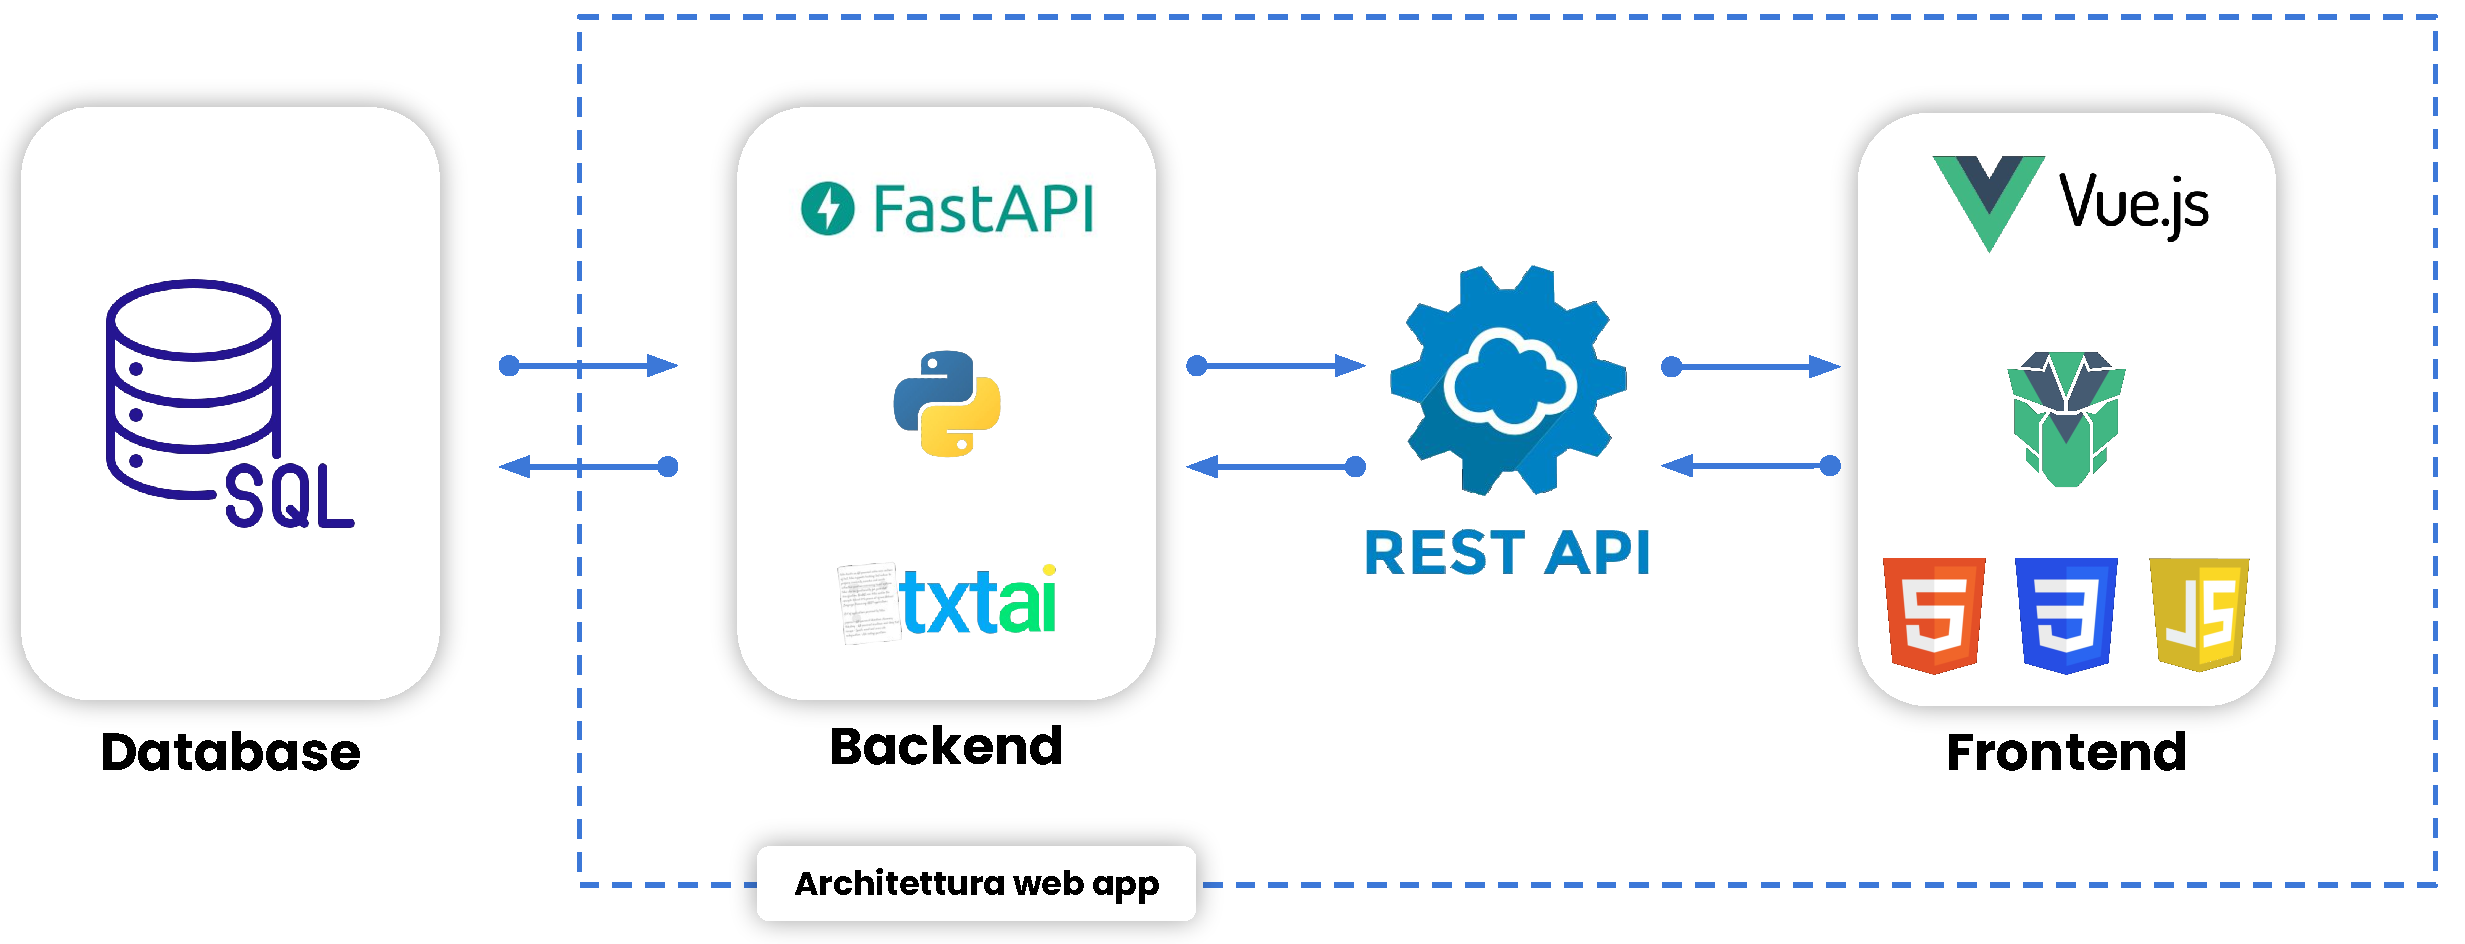
\includegraphics[width=\textwidth]{assets/architettura_web_app.pdf}
  \caption{Architettura web app}
\end{figure}

\subsection{Assemblaggio dei componenti}
\par Docker Compose viene utilizzato per gestire applicazioni multi-container, permettendo di assemblare diversi servizi che compongono un'applicazione. Nel contesto di ChatSQL, il team ha creato i seguenti container Docker:
\begin{itemize}
  \item \textbf{backend}: espone l'interfaccia di backend sulla porta 8000. All'indirizzo \textit{localhost:8000/docs} è possibile consultare la documentazione interattiva delle API. Inoltre, sono disponibili dettagli sui Data Transfer Objects (DTO);
  \item \textbf{frontend}: espone l'interfaccia utente sulla porta 5173.
\end{itemize}

\subsection{Struttura del sistema}

\par Il modello architetturale scelto dal gruppo è il modello ad \textbf{architettura esagonale}. Questo modello trova le sue basi nell'architettura a livelli, dalla quale cerca di prenderne le basi e di far fronte ai problemi di dipendenza stretta che si creavano tra i livelli.
\par L'architettura è composta da 3 parti principali:
\begin{itemize}
    \item \textbf{Core}: il core è la sezione centrale dell'architettura, in cui risiede la business logic dell'applicazione. È indipendente da qualsiasi interfaccia utente o servizio esterno. Ciò viene fatto per mantenerla isolata e disaccoppiata dal resto dell'architettura, in modo che possa agire indipendentemente;
    \item \textbf{Port}: costituiscono dei punti di comunicazione tra il core e altri parti del sistema o servizi esterni. Esistono due tipi principali di porte:
    \begin{itemize}
        \item Inbound port: consentono al nucleo di essere invocato da componenti esterne;
        \item Outbound port: consentono al nucleo di reperire informazioni dall'esterno.
    \end{itemize}
    \item \textbf{Adapter}: sono pattern architetturali che permettono di adattare i dati in modo che possano essere ricevuti dall'esterno e passare per le porte o vice versa. Costituiscono la sezione più esterna dell'architettura e consentono pertanto il passaggio e il monitoraggio dei dati.
\end{itemize}

\vspace{0.5\baselineskip}
\par Questa architettura è rappresentata a forma esagonale per diversi motivi; da una parte l'architettura vuole ricordare la cella di un alveare. Avendo tale forma, la cella si può incastrare con altre celle allo scopo di definire un alveare. Allo stesso modo un'architettura esagonale può interfacciarsi con altre strutture con le stesse caratteristiche per definire un sistema più grande. Un altro motivo della scelta è la visualizzazione della simmetria della struttura, la quale viene visualmente divisa a metà, dove una metà si interfaccia con l'esterno per ricevere gli input, mentre l'altra si interfaccia con l'esterno per inviare informazioni in output.
\par L'architettura esagonale offre numerosi vantaggi, tra i quali:
\begin{itemize}
    \item \textbf{Flessibilità}: i componenti dell'architettura agiscono indipendentemente tra di loro e di conseguenze si possono adattare con facilità;
    \item \textbf{Scalabilità}: una cella ad architettura esagonale può essere vista come un microservizio e per tanto risulta più facilmente replicabile;
    \item \textbf{Testabilità}: il core è isolato e disaccoppiato dal resto dell'architettura;
    \item \textbf{Manutenibilità}: in quanto il core è isolato e disaccoppiato dal resto dell'architettura.
\end{itemize}

\vspace{0.5\baselineskip}
\par Questo tipo di architettura non è immune a difetti, tra i quali si possono trovare:
\begin{itemize}
    \item \textbf{Complessità}: l'architettura richiede una progettazione puntuale e una buona conoscenza dei pattern architetturali;
    \item \textbf{Dipendenza} che permane tra il core e le porte: cambiamenti sostanziali del core possono richiedere una manutenzione delle porte;
    \item \textbf{Difficoltà di debugging}: il core è separato dal resto dell'architettura, di conseguenza è possibile introdurre \glossario{bug} nell'integrazione con servizi esterni.
\end{itemize}

\vspace{0.5\baselineskip}
\par Il gruppo ha concordato di adottare questo modello architetturale, poiché ritiene che il core dell'applicazione sia sufficientemente robusto da non dover creare problemi di manutenzione nel tempo. Inoltre, la scalabilità e la flessibilità di questo modello architetturale sono state considerate un vantaggio significativo per gestire la varietà dei contesti di applicazione del sistema. Infine, l'architettura si sposa bene con le esigenze dell'applicazione di interfacciarsi con servizi esterni quali \glossario{database} o \glossario{LLM} e \glossario{API}.
\subsubsection{Back-end}

\par La struttura organizzativa del back-end segue i principi dello stile architetturale scelto, al fine di semplificare il processo di traduzione della progettazione in codice. Il back-end è suddiviso nelle seguenti cartelle:

\begin{minipage}{\textwidth}
  \dirtree{%
    .1 backend.
    .2 TODO.
    .2 TODO.
  }
\end{minipage}
\subsubsection{Back-end}

\par La struttura organizzativa del back-end segue i principi dello stile architetturale scelto, al fine di semplificare il processo di traduzione della progettazione in codice. Il back-end è suddiviso nelle seguenti cartelle:

\begin{minipage}{\textwidth}
  \dirtree{%
    .1 backend.
    .2 TODO.
    .2 TODO.
  }
\end{minipage}
